\section{Auswertung}

\subsection{Datenanalyse}
Die gemessenen Daten des Beschleunigungssensors werden in $m/s^{2}$ 
dargestellt, die Daten des Gyroskopes in $\circ/s$ ($\circ$:  Grad).

Die Analyse wird durch zwei Faktoren erschwert:
\begin{enumerate}
	\item Die Sensoren sind sehr empfindlich.
	\item Baulich bedingt dreht sich das Ei sehr leicht um die Längsachse, wodurch eine kurze Beschleunigung auf eine konstante Geschwindigkeit nicht als ein einzelner Ausschlag, sondern als eine Kombination verschiedener, dargestellt wird und so kaum erkennbar ist.
\end{enumerate}

Da bisher noch kein Klassifikator existiert, wird die Auswertung von Hand durchgeführt. Um dies zu erleichtern, wurde ein Savitzky-Golay-Filter mit den Parameterpaaren (25, 5) und (75,7) eingesetzt. Die Werte beschreiben in dieser Form (Fenstergröße, Grad des Polynoms) die Eingangsparameter für den Filter. Denn bei direktem visuellen Vergleich zweier Testläufe über den kompletten Zeitverlauf, werden die Graphen zusammengestaucht und Bewegungstendenzen sind dadurch schwerer zu erkennen und zu bewerten. Der Einsatz eines Filters dient an dieser Stelle der Erleichterung, die Einteilung des Graphen in verschiedene Segmente vorzunehmen. \\
Ob die Verwendung eines Filters auch geeignet beziehungsweise notwendig ist, um Messrauschen aus den Daten zu entfernen, muss noch geprüft werden.

In Abbildung \ref{fig:k5_segmentierung} wurde der Datensatz Nr. 1 mit einer Länge von 3,3 Minuten untersucht\footnote{Anmerkung: Der Client visualisiert die Daten in einer anderen Farbkombination. Die Abbildungen \ref{fig:k5_segmentierung} und \ref{fig:k5_segmente_vergleich} wurden nachträglich für eine besser erkennbare Darstellung im Dokument eingefärbt.}. Die oberen beiden Graphen zeigen die ungefilterten Beschleunigungswerte und Winkelgeschwindigkeiten der Rohdaten, wogegen die unteren beiden Graphen den gleichen Datensatz mit angewendetem Savitzky-Golay-Filter (75,7) zeigen. Auf der x-Achse sind die Datentupel aufgetragen, wobei alle 86 Millisekunden ein neuer Datensatz empfangen wurde.

\begin{figure}[htb]
	\centering
	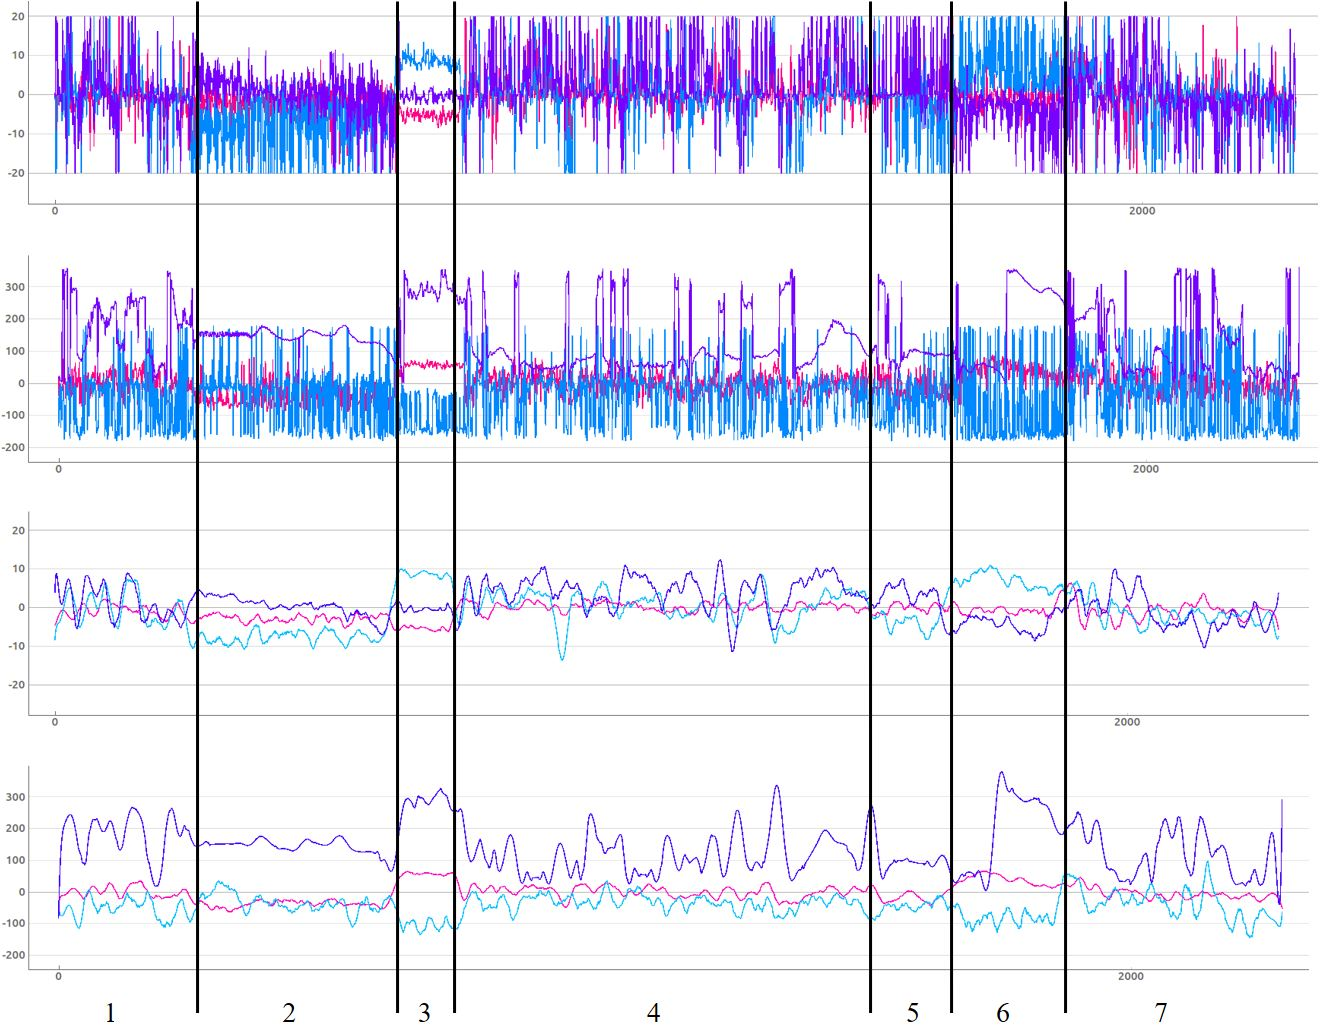
\includegraphics[width=1\linewidth]{images/k5-segmentierung.JPG}
	\caption{Datenanalyse: Nummerierte Segmentierung des ersten Datensatzes; Dargestellte Graphen: 1) Beschleunigungsdaten im Rohformat, 2) Winkelgeschwindigkeiten im Rohformat, 3)  Beschleunigungsdaten mit angewendetem Savitzky-Golay-Filter (75,7), 4) Winkelgeschwindigkeiten mit angewendetem Savitzky-Golay-Filter (75,7)}
	\label{fig:k5_segmentierung}
\end{figure}

Die Segmentierungen wurden an den Stellen gesetzt, an denen sich stärkere Änderungen bei den Bewegungsmustern erkennen lassen. Die Anzahl der Anlagenmodule ist bekannt. Da ein Messlauf mitten in einem Modul startet und endet, da die Anlage einen geschlossenen Schüttgut-Kreislauf hat, sind sieben Segmente notwendig. Das erste und letzte Segment gehören dabei zum selben Modul. Diese lassen sich wie folgt zu den einzelnen Anlagenmodulen zuordnen und beschreiben:

\begin{description}
	\item [1 Großer Rüttler unten:] Der Rüttler hat eine hohe Rüttelstärke, weshalb die Schüttgüter auf diesem stark springen. Dies lässt sich anhand den schwankenden Graphen sowohl bei der Beschleunigung als auch bei der Winkelgeschwindigkeit erkennen. Da ein Rundenlauf der Kapsel in diesem Modul startet und endet, ist das Bewegungsmuster sehr ähnlich zu dem in Segment 7.
	\item [2 Querförderband unten:] Auf dem Förderband liegt das Schüttgut ruhig. Die Graphen haben geringere Ausschläge. 
	\item [3 Förderband nach oben:] Das Förderband bewegt das Schüttgut schnell nach oben, weshalb dieses Segment sehr kurz ist. Zudem ist dieses Förderband sehr steil und besitzt daher Mitnehmstützen, sodass das Schüttgut nicht nach unten rollen kann, sondern ruhig liegen bleibt. Hier sind die geringsten Ausschläge zu erkennen.
	\item [4 Mittlerer Rüttler, quer oben:] Auf diesem Rüttler sind die Ausschläge für Beschleunigung und Winkelgeschwindigkeit wieder wesentlich stärker
	\item [5 Kurzer Rüttler:] Der kurzer Rüttler gibt das Schüttgut für das Sortierband frei und hat eine geringere Rüttelstärke als andere, wodurch sich das Schüttgut ruhig vorwärts schiebt, statt zu springen.
	\item [6 Rutsche und Sortierband] Über die Rutsche fällt das Schüttgut auf das Sortierband, welches das Schüttgut mit 3 $m/s$ befördert. Die Beschleunigungsdaten schwanken hier weniger stark, wobei es einen Peak in einer Achse der Winkelgeschwindigkeiten gibt und es zu zwei Vorzeichenänderungen in den Beschleunigungswerten kommt.   
	\item [7 Großer Rüttler unten:] Siehe Erklärung für Segment 1.	
\end{description}

Nachdem Segmente gefunden wurden, in denen es unterschiedliche Bewegungsmuster gibt, müssen diese mit den weiteren Datensätzen von anderen Messläufen evaluiert werden. Abbildung \ref{fig:k5_segmente_vergleich} zeigt einen Vergleich der Segmente zwischen Datensatz 1 (Dauer: 3,3 Minuten) und Datensatz 17 (Dauer: 2,4 Minuten). 

\begin{figure}[htb]
	\centering
	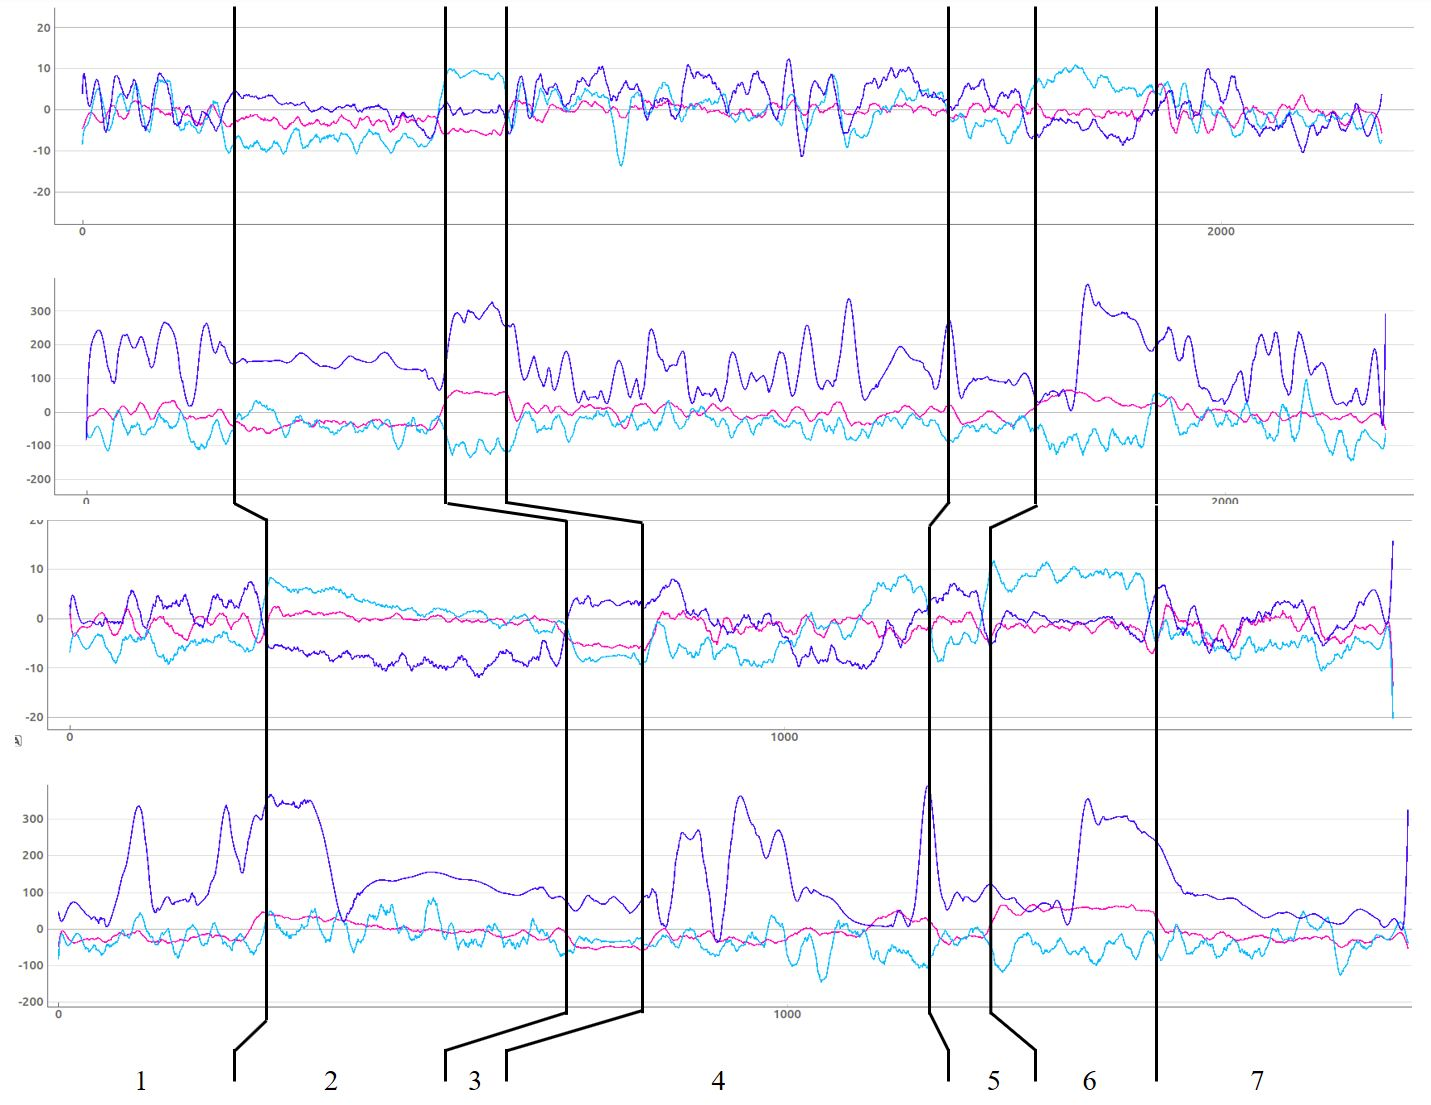
\includegraphics[width=1\linewidth]{images/k5-segmente_vergleich.JPG}
	\caption{Datenanalyse: Vergleich der gefundenen Segmente von zwei verschiedenen Datensätzen (1 + 17), jeweils mit angewandtem Savitzky-Golay-Filter (75,7); Dargestellte Graphs: 1) Datensatz 1, Beschleunigungsdaten, 2) Datensatz 1, Winkelgeschwindigkeiten, 3) Datensatz 17, Beschleunigungsdaten, 4) Datensatz 17, Winkelgeschwindigkeiten}
	\label{fig:k5_segmente_vergleich}
\end{figure}

Anhand der oben beschriebenen Verhaltensmustern lassen sich die Segmente auch in Datensatz 17 in der gleichen Reihenfolge erkennen. Vor allem deutlich sichtbar werden die unterschiedlichen Muster zwischen Rüttler (stark schwankend; 1, 4, 5, 7) und Förderbändern (ruhiger; 2, 3, 6). Besonders markant ist Segment 3, das auch in den Rohdaten durch geringe Schwankungen in den Messwerten deutlich hervor- und auch in ähnlicher Abschnittslänge auftritt. Bei den Rüttlermodulen kann es passieren, dass die Kapsel nicht gut vom Schüttgut mitgenommen wird und mehr Zeit benötigt. Der Übergang zu Segment 5 wird mit einem höheren Ausschlag im Winkelgeschwindigkeits-Graphen begonnen. Bei diesem Anlagenabschnitt fällt die Kapsel etwa einen halben Meter auf den nächsten Rüttler. In Segment 6 lässt sich immer ein stärkerer Peak bei der Winkelgeschwindigkeit finden, der dann langsam abfällt.
Der Übergang von Segment 5 auf Segment 6 kann allerdings nicht exakt ausgewertet werden. Es gibt zwar an diesen Stellen Änderungen in der Bewegungstendenz, allerdings ist die Zeitdauer von Segment 6 für Rutsche und Sortierband unerwarteterweise unterschiedlich lang. An dieser Stelle wurden die Daten nie in eine Datei zwischengespeichert.

Die händisch vorgenommene Segmentierung wurde mittels den erstellten Datendateien beim Zwischenspeichern der Android-App an den markanten Punkten kontrolliert.

\subsection{Evaluation der Methode}
Es hat sich gezeigt, dass einzelne Segmente in den Daten erkennbar sind, die sich mit den Modulen der Anlage korrelieren lassen. In Kombination mit dem beobachteten Verhalten des instrumentierten Schüttguts auf der Bahn können diese Erkenntnisse auch auf das zu sortierende Schüttgut übertragen werden. 

Mit Hilfe des instrumentierten Schüttguts lassen sich beispielsweise Verweilzeiten auf den einzelnen Anlagenmodulen bestimmen. Durch Anpassung der Anlagenparametern wie Geschwindigkeiten von Förderbändern oder Rüttlerstärke können die Auswirkungen auf die Schüttgüter durch erneut gemessene Daten überprüft werden.

Zusätzlich können mit Hilfe von instrumentierten Schüttgütern Aussagen über das Bewegungsverhalten des Schüttguts selbst gemacht werden, sofern die Abweichungen in Größe, Oberflächenbeschaffenheit und Gewicht nicht zu groß sind. Damit könnten vielleicht Bewegungsmodelle für Schüttgüter gewonnen werden.

\subsection{Fazit}

Es konnte ein instrumentiertes Schüttgut entwickelt werden, mit dem Beschleunigungs- und Orientierungsdaten gemessen werden können. Die gewählten Bauteile von Adafruit passen im gelöteten Zustand in eine Ü-Ei-Kapsel. Die Bluetoothverbindung wird durch die Kapsel selbst nicht beeinträchtigt. Jedoch befindet sich an der Anlage ein großer Anteil Metall, was sich unter Umständen auch negativ auf die Bluetoothverbindung auswirkt. Durch Nutzung einer Android-App kann jedoch auf Höhe des Sensors an der Anlage mitgelaufen werden. Die Hardware des Mikrocontrollers weist noch Schwachstellen auf. Darunter fallen insbesondere die empfindlichen Lötverbindungen an den einzelnen Platinen, die z.B. durch Vibrationen in der Kapsel brechen können. Ebenso sind bei Nutzung mehrerer Mikrocontroller Referenzmessungen notwendig, um unterschiedliche Verhaltensarten der Mikrocontroller frühzeitig zu identifizieren. Eine besondere Rolle spielt hier vor allem die Taktung des Adafruit-Mikrocontrollers, durch den die Anzahl der gemessenen Datentupel in einem Zeitraum bestimmt werden.

Die Verpackung der Kapsel wirkt sich bei einem Messlauf auf das Bewegungsverhalten aus. Mit der Polsterfolie gewinnt das instrumentierte Schüttgut an Größe. Die Erweiterung mit Flügeln wirkt sich positiv auf die Geschwindigkeit aus, sie dienen als Mitnahmemöglichkeit durch das umliegende Schüttgut. Gegenüber dazu stellen sich die Messreihen mit Kapsel ohne Verpackung und im Alurahmen. Neben der geänderten Form durch die Aluverpackung sind die Oberflächen sehr viel glatter und unähnlicher zu den Steinen. 
Abgesehen vom Verpackungstyp ist die Kapsel mit ihrer Originalgröße größer bzw. im Verhältnis zu Steinen der gleichen Größe wesentlich leichter. Dadurch erfährt die Kapsel in der Steinmenge einen höheren Auftrieb und spiegelt nicht exakt das Bewegungsmuster des Schüttguts, in diesem Fall der Steine, wieder. 

Der Client kann die gewonnen Daten aufbereiten und visuell darstellen. Implementiert wurde ein Savitzky-Golay-Filter, der bei der Datenanalyse genutzt wurde. Die Filterparameter sind hier experimentell ermittelt, wodurch die Eignung anhand weiterer Daten verifiziert werden muss. Allerdings sollte bei erweiterten Auswertungen evaluiert werden, in wie weit die Nutzung des Filters sinnvoll ist. \\
Die gewonnen Daten sind jedoch mit Vorsicht zu betrachten, da die Messläufe unterschiedlich lang sind und Verbindungsabbrüche auftreten können. 

Aus der Datenanalyse ging hervor, dass sich bestimmte Bewegungsmuster in immer gleich auftretender Reihenfolge in den Messläufen erkennen lassen. Anhand bestimmten charakteristischen Mustern in Segmenten lässt sich eine Zuordnung zu den Anlagenmodulen vornehmen. 

\subsection{Ausblick}

Wie sich gezeigt hat, sind noch einige Erweiterungen und Optimierungen möglich. 
Im Bereich des Mikrocontrollers könnte statt einer Bluetooth-Verbindung eine Speicherkarte hinzugefügt werden, aus der die Daten am Laptop ausgelesen werden. Dies hätte den Vorteil, dass keine Daten durch Verbindungsabbrüche verloren gehen können. Allerdings würde dadurch auch die Kontrolle über den Mikrocontroller verringert, da keine Befehle, wie z.B. das Zurücksetzen von Zählen zum Markieren einer neuen Messrunde, gesendet werden könnten. In diesem Fall müsste man entweder nach jedem Lauf die Daten aus dem Mikrocontroller auslesen oder eine Segmentierungsmethode finden, um eine große Datei, die mehrere Messläufe enthält, in einzelne Dateien zu separieren, die dann jeweils nur noch einen Messlauf beinhalten. \\
Unter Umständen ließe sich das Probleme der auftretenden Verbindungsabbrüchen lösen, indem ein anderes Funkmodul wie beispielsweise WLAN verwendet wird. Allerdings ist dabei nicht bekannt, wie sich die Metallwände des FlexSorts auf diese Verbindungsart auswirkt.\\
Um eine größere Verlässlichkeit der Messergebnisse zu erreichen und das Verhalten der Schüttgüter untereinander besser zu beobachten, könnten parallele Messungen mit mehreren instrumentierten Schüttgütern vorgenommen werden. Dazu müsste entweder die App noch erweitert werden, sodass Verbindungen zu mehreren Mikrocontrollern möglich sind oder die Mikrocontroller mit internem Speicher ausgestattet werden, sodass keine Verbindung zum Speichern der Daten mehr notwendig ist.

Auch bei der App sind noch Optimierungsmöglichkeiten beziehungsweise mögliche Erweiterungen denkbar. Um die Auswertung am PC komfortabler zu gestalten, könnte eine direkte Datenübertragung an den PC implementiert werden, sodass die Daten nicht zuerst manuell vom Smartphone, eventuell noch über einen Cloudspeicher, auf den Laptop übertragen werden müssen. 
Ein nützliches Feature wäre ein Live-Graph, der die empfangenen Daten sofort in der App visualisiert.\\
Eventuell ist es möglich, die empfangenen Daten am Smartphone direkt über einen Data-Service an einen PC zu streamen, an dem weitere Analysen gemacht werden. In Verbindung mit einer Visualisierung gäbe es dann die Möglichkeit, direkt in Echtzeit Aussagen zum Aufenthalt der Kapsel in der Anlage machen zu können. 

Beim Client wäre die wichtigste Erweiterung der bereits erwähnte Klassifikator. Dabei bleibt noch zu evaluieren, ob ein supervised oder unsupervised Ansatz gewählt werden soll und welche Art von Klassifikator an sich geeignet ist. Sollte ein supervised Klassifikator gewählt werden, wäre für eine bessere Segmentierung eines Messlaufs mit Zuordnung auf die einzelnen Anlagenmodulen der Einsatz von RFID-Schranken an den entsprechenden Übergängen der Module nützlich. So wäre die Segmentierung deutlich präziser. Unabhänging davon, welcher Ansatz nun letztendlich verfolgt wird, müssen wesentlich mehr Daten gemessen werden.
Eine andere mögliche Erweiterung des Clients, ist eine Darstellung der Graphen oder auch eine Simulation in 3D, wie sich der Mikrocontroller im Raum bewegt.